\subsection{Amministratore}

\subsubsection{Panoramica Amministratore}
\begin{figure}[H]
\centering
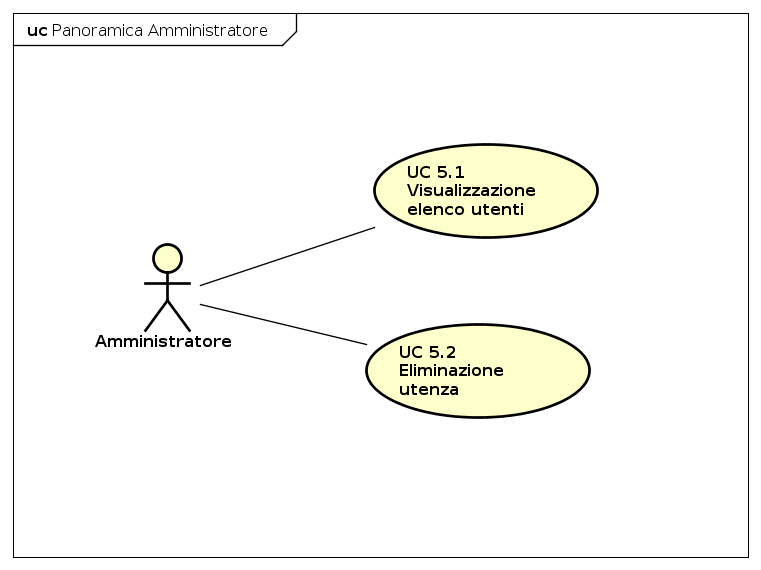
\includegraphics[width=17cm, height=10cm]{img/PanoramicaAmministratore.png} 
\caption{Panoramica Amministratore}
\end{figure}


\subsubsection{UC 5.1 - Visualizzazione della propria dashboard}


\begin{figure}[H]
\centering
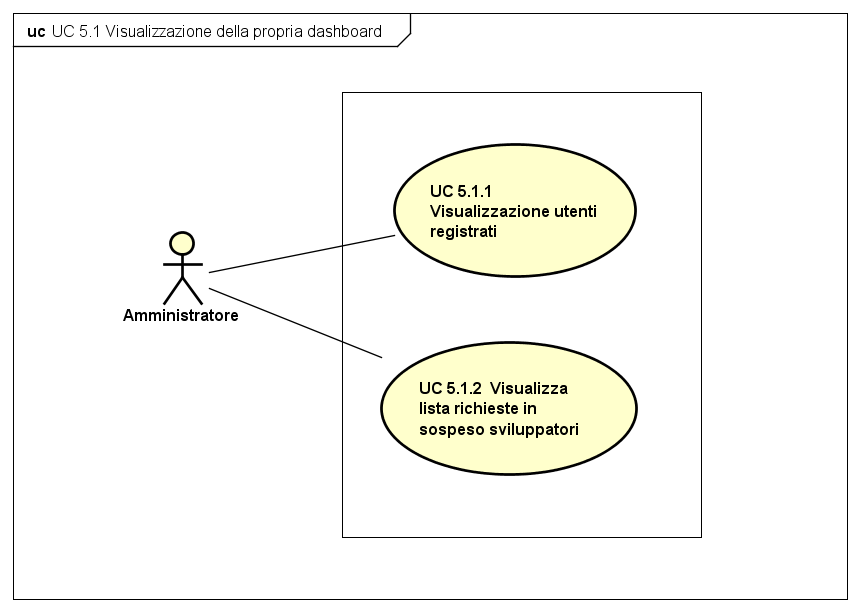
\includegraphics[width=17cm, height=10cm]{img/UC51.png} 
\caption{Caso d'uso UC 5.1}
\end{figure}


\begin{itemize}
\item[•] \textbf{Attore}: Amministratore; 
\item[•] \textbf{Descrizione}: L'amministratore accede alla propria dashboard personale e può effettuare modifiche al sistema;
\item[•] \textbf{Precondizione}: Il sistema offre la possibilità di accedere alla propria dashboard;
\item[•] \textbf{Postcondizione}: L'amministratore è all'interno della sua dashboard;
\item[•] \textbf{Flusso degli eventi}:

\begin{enumerate}
\item UC 5.1.1 Visualizzazione utenti registrati;
\item UC 5.1.2 Visualizza lista richieste in sospeso sviluppatori.
\end{enumerate}

\end{itemize}
\subsubsection{UC 5.1.1 - Visualizzazione utenti registrati}

\begin{figure}[H]
\centering
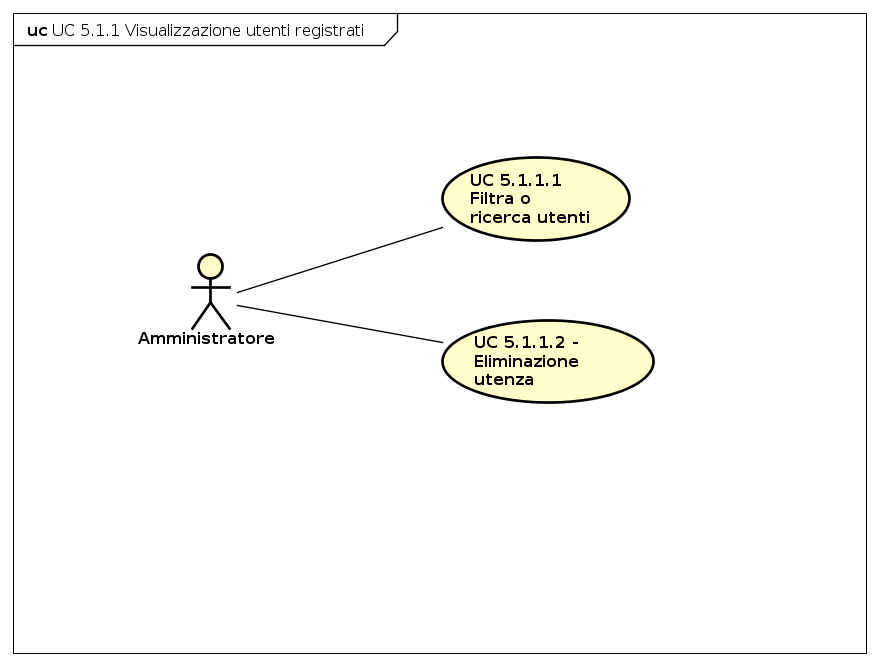
\includegraphics[width=17cm, height=10cm]{img/UC511.png} 
\caption{Caso d'uso UC 5.1.1}
\end{figure}


\begin{itemize}
\item[•] \textbf{Attore}: Amministratore;

\item[•] \textbf{Descrizione}: L'amministratore visualizza l'elenco degli utenti registrati nel sistema;

\item[•] \textbf{Precondizione}: L'amministratore si è autenticato nel sistema e visualizza la propria dashboard;

\item[•] \textbf{Postcondizione}: L'amministratore visualizza la lista di utenti registrati al sistema; 

\item[•] \textbf{Flusso degli eventi}:

% L'amministratore accede alla pagina contenente l'elenco degli utenti e visualizza i dati degli utenti. 

\begin{enumerate}

\item UC 5.1.1.1 - Filtra utenti;
\item UC 5.1.1.2 - Visualizza dettaglio utente.

\end{enumerate}

	\item[•] \textbf{Estensioni}:	
\begin{enumerate}
	\item UC 5.1.1.2.1 - Eliminazione utenza.
\end{enumerate}

\end{itemize}

\subsubsection{UC 5.1.1.1 - Filtra utenti}
\begin{itemize}

\item[•] \textbf{Attore}: Amministratore;
\item[•] \textbf{Descrizione}: L'amministratore ha la possibilità di ricercare gli utenti a partire dal loro nome o dalla loro tipologia di utenza;
\item[•] \textbf{Precondizione}: Il sistema offre la possibilità di filtrare o cercare gli utenti a seconda del loro nome o della loro tipologia di utenza;
\item[•] \textbf{Postcondizione}: Il sistema visualizza gli utenti selezionati.

\end{itemize}

\subsubsection{UC 5.1.1.2 - Visualizza dettaglio utente}
\begin{itemize}
	
	\item[•] \textbf{Attore}: Amministratore;
	\item[•] \textbf{Descrizione}: L'amministratore ha la possibilità di visualizzare in dettaglio un utente specifico
	\item[•] \textbf{Precondizione}: Il sistema offre la possibilità di visualizzare i dati privati degli utenti;
	\item[•] \textbf{Postcondizione}: Amministratore ha visualizzato informazioni personali utente.
	
\end{itemize}


\subsubsection{UC 5.1.1.2.1 - Eliminazione utenza}
\begin{itemize}
\item[•] \textbf{Attore}: Amministratore;
\item[•] \textbf{Descrizione}: L'amministratore elimina un'utenza dal sistema;
\item[•] \textbf{Precondizione}: L'amministratore \`{e} autenticato e visualizza l'elenco degli utenti registrati nel sistema ed ha selezionato un utente da eliminare;
\item[•] \textbf{Postcondizione}: L'amministratore ha eliminato l'utenza dal sistema; 
\item[•] \textbf{Flusso degli eventi}:

\begin{enumerate}
%\item Selezione utente;
\item Conferma eliminazione utente;
\item Annulla eliminazione.
\end{enumerate}
\end{itemize}


\subsubsection{UC 5.1.2 - Visualizza lista richieste in sospeso sviluppatori}
\begin{itemize}

\item[•] \textbf{Attore}: Amministratore;
\item[•] \textbf{Descrizione}: L'amministratore visualizza tutti gli utenti che si vogliono registrare come sviluppatori nel sistema e può accettare o no l'iscrizione;
\item[•] \textbf{Precondizione}: Il sistema offre la possibilità di visualizzare la lista degli utenti che si vogliono registrare come sviluppatori;
\item[•] \textbf{Postcondizione}: L'amministratore visualizza la lista delle richieste in sospeso;
\item[•] \textbf{Flusso degli eventi}:
\begin{enumerate}
\item Accetta sviluppatore;
\item Rifiuta sviluppatore.
\end{enumerate}

\end{itemize}

